\documentclass[11pt]{beamer}
\usepackage[utf8]{inputenc}
\usepackage{amsmath}
\usepackage{algpseudocode}
\usepackage{algorithm}
% \usepackage{algorithm,algorithmic}
% \usepackage{animate}

%Information to be included in the title page:
\title{Max Integral Operator: A Probabilistic Numeric Approach}
\author{Nishad Gothoskar}
\institute{Learning and Intelligent Systems - MIT}
\date{August 25 2018}
 
 
\begin{document}
 
\frame{\titlepage}
 
 \begin{frame}
 \frametitle{Motivation}
Bellman Update in Continuous State-Action Spaces
 \[V^{\pi}(x) = \max_{u \in A} \int_{x' \in S} p(x'|u)\big(R(x'|x,u) + \gamma^{\Delta t}V^{\pi}(x')\big) \ \textup{d}x' \]
 
 Use a GP to model the Value Function
 
\end{frame}


\begin{frame}
\frametitle{Max Integral Operator}
In this work, we will explore techniques to evaluate expressions of the following form:
\begin{equation*}
    \max_{a} \int f(s', a) p(s', a) \ \text{d}s'
\end{equation*}
\newline
We find the Max Integral expression in a variety of computational problems.
\hfill \newline
Intuitively, maximizing over some parameters while integrating out others is a useful operation.
\end{frame}

\begin{frame}
\frametitle{Problem Formulation}
\begin{itemize}
	\item We consider functions $f$ for which the following integral converges for all $a$.
	\begin{equation*}
	\int_{- \infty}^{\infty} f(a,s) p(s) \ \text{d}s
	\end{equation*}
	\item $s$ is a continuous parameter
	\item $a$ may be either continuous or discrete
	
\end{itemize}

\end{frame}

\begin{frame}
\frametitle{Preliminaries}
\begin{itemize}
	\item Bayesian Optimization
	\item Bayesian Quadrature
\end{itemize}
\end{frame}

\begin{frame}
\frametitle{Bayesian Quadrature}
Most work in BQ has focused on integrals of the form:
\begin{equation*}
\int f(x) p(x)  \ \text{d}x
\end{equation*}
First presented as Bayes-Hermite Quadrature [1], BQ uses active sampling to estimate an integral's value. This is done by using a Gaussian Process to model the integrand and then integrating the GP.
\newline\newline
This gives us an estimated mean and variance for the integral's value.
\end{frame}

\begin{frame}
\frametitle{Bayesian Quadrature - Acquisition Function}
To sample function evaluations we optimize:
\begin{equation*}
\begin{split}
\bar{f} &= \int f(x)p(x)dx\\
x^{*} &= \operatorname*{argmin}_{x} \mathbb{V}(\bar{f} | \mathcal{D},\boldmath{x})
\end{split}
\end{equation*}
\begin{figure}
	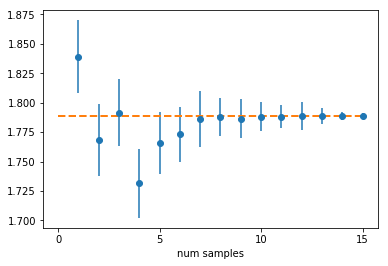
\includegraphics[width=0.5\textwidth]{converge}
\end{figure}
\end{frame}


\begin{frame}
\frametitle{Bayesian Quadrature - Closed Form}
\begin{equation*}
\begin{split}
&\int (k(s,\boldmath{x}) K^{-1}\boldsymbol{f}) \ p(s) ds = z^{T} K^{-1}\boldsymbol{f} \\
&z_i = \int exp(-0.5 \sum_{d=1}^{D}\frac{(s_d - x^{(i)}_d)^2}{w_d^2} )\ exp(-0.5 \sum_{d=1}^{D}\frac{s_d^2}{\sigma_d^2} )\prod_{d=1}^{D} 2 \pi \sigma_d ds\\
&z_i = \int exp(-0.5 \sum_{d=1}^{D}\frac{\sigma_d^2(s_d - x^{(i)}_d)^2 + w_d^2 s_i^2}{w_d^2 \sigma_d^2} )\prod_{d=1}^{D} 2 \pi \sigma_d ds\\
&z_i = \int exp(-0.5 \frac{(x^{(i)}_d)^2}{w_d^2 + \sigma_d^2}) \prod_{d=1}^{D} (2 \pi \frac{w_d^2 + \sigma_d^2}{w_d^2 \sigma_d^2} )^{-1/2}  \prod_{d=1}^{D} 2 \pi \sigma_d ds\\
&z_i = \int exp(-0.5 \sum_{d=1}^{D} \frac{(x^{(i)}_d)^2}{w_d^2 + \sigma_d^2}) \prod_{d=1}^{D} (\frac{w_d^2 + \sigma_d^2}{w_d^2} )^{-1/2} ds \\
\end{split}
\end{equation*}
\end{frame}

\begin{frame}
\frametitle{Bayesian Quadrature - Closed Form}
\begin{equation*}
\begin{split}
&\int k(s,\boldmath{x})p(s) ds = r \\
&r_i = \int exp(-0.5 \sum_{d=1}^{D}\frac{(s_d - x^{(i)}_d)^2}{w_d^2} )\ exp(-0.5 \sum_{d=1}^{S}\frac{s_d^2}{\sigma_d^2} )\prod_{d=1}^{S} 2 \pi \sigma_d ds\\
&r_i = exp(-0.5 \sum_{d=S+1}^{D}\frac{(s_d - x^{(i)}_d)^2}{w_d^2} )\ z_i\\
\end{split}
\end{equation*}
\end{frame}

\begin{frame}
\frametitle{Bayesian Optimization}
\begin{equation*}
x^{*} = \operatorname*{argmax}_{x} f(x)
\end{equation*}
Model $f$ and use GP posterior mean and variance to select queries.
\begin{equation*}
\mu(x) + \beta \sigma (x)
\end{equation*}
For Max Integral Optimization, we apply UCB to selecting $a$.   
\newline \newline
$\mu$ and $\sigma$ are from estimating the integral.
\end{frame}

\begin{frame}
\frametitle{Method}
Our method resembles Bayesian Optimization and Bayesian Quadrature, because we sample to both reduce uncertainty of the inner integral and find the maximum value $a$.
\newline \newline
However, by considering both these objectives and using an acquisition function that accurately captures them, we can converge with fewer function evaluations.
\end{frame}

\begin{frame}
\frametitle{Method}
\begin{figure}
	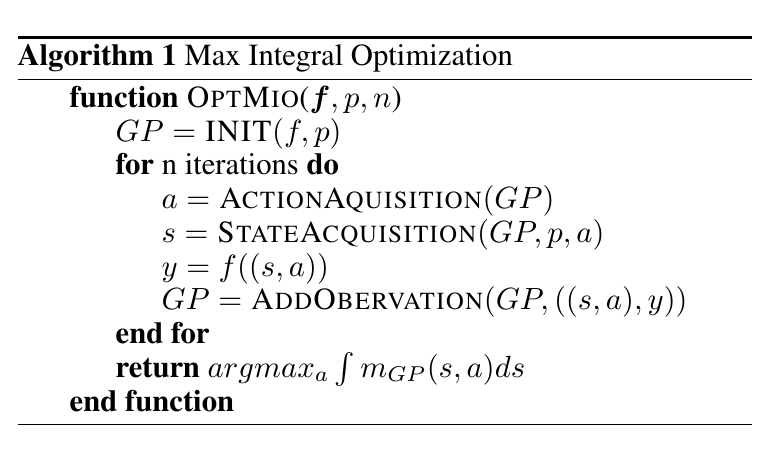
\includegraphics[width=0.8\textwidth]{alg2}
\end{figure}
\end{frame}


\begin{frame}
\frametitle{Experiments}
\begin{itemize}
	\item Synthetic Functions
	\item Reinforcement Learning
\end{itemize}
\end{frame}


\begin{frame}
\frametitle{Synthetic Functions}
We first demonstrate our method on random functions drawn from a Gaussian Process.
\newline \newline
We evaluate settings with 1 or 2 dimensional action space and up to 3 dimensions state spaces.
\end{frame}

\begin{frame}
\frametitle{Synthetic Functions}
\begin{figure}
	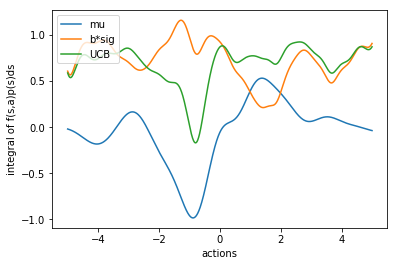
\includegraphics[width=0.6\textwidth]{3}
\end{figure}
UCB on actions represents a confidence bound on the integral estimate (along that action dimension).
\end{frame}

\begin{frame}
\frametitle{Synthetic Functions}
\begin{figure}
	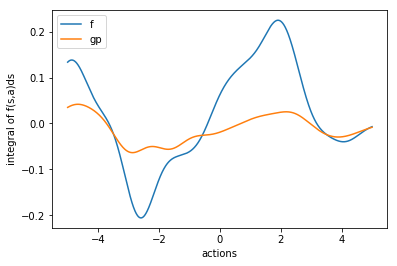
\includegraphics[width=0.55\textwidth]{2}

	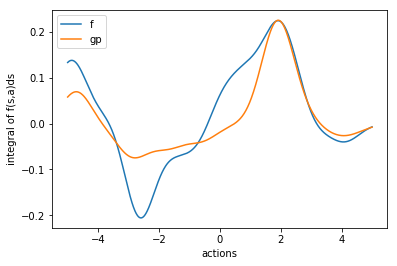
\includegraphics[width=0.55\textwidth]{1}
\end{figure}
\end{frame}

\begin{frame}
\frametitle{Reinforcement Learning}
We can apply these methods to the Bellman Update:
 \[V^{\pi}(x) = \max_{u \in A} \int_{x' \in S} p(x'|u)\big(R(x'|x,u) + \gamma^{\Delta t}V^{\pi}(x')\big) \ \textup{d}x' \]

This setting differs from the synthetic functions because now $p$ depends on the action.
\newline \newline

We are working on using this for Value Iteration and RTDP.
\end{frame}

\begin{frame}
\frametitle{Reinforcement Learning}
\begin{figure}
	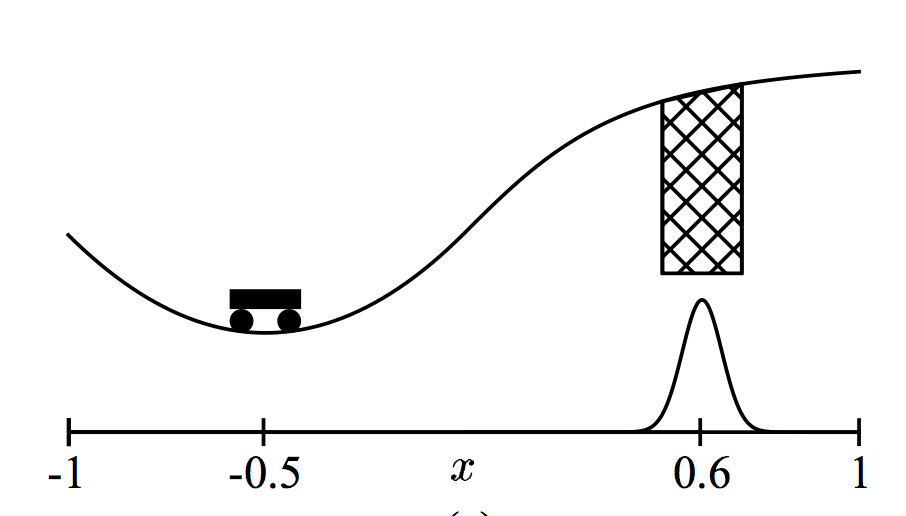
\includegraphics[width=0.5\textwidth]{mcar}
\end{figure}
Rasmussen and Kuss (2004) use GP to model:
\begin{itemize}
	\item System Dynamics
	\item Value Function 
\end{itemize}
And this defines an implicit policy:
\begin{figure}
	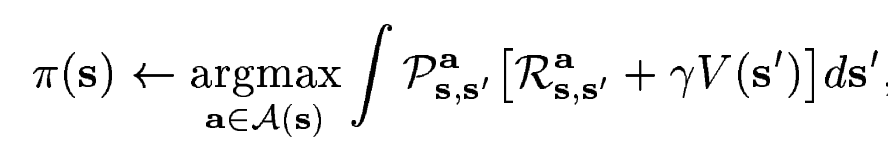
\includegraphics[width=0.6\textwidth]{integral}
\end{figure}
\end{frame}

\begin{frame}
\frametitle{Reinforcement Learning}
\begin{figure}
	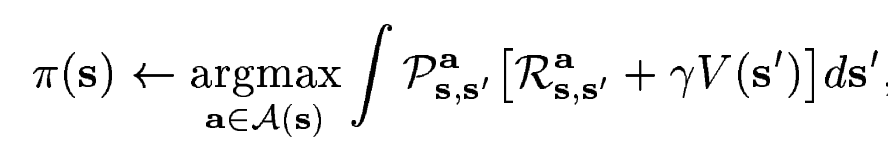
\includegraphics[width=0.6\textwidth]{integral}
\end{figure}
Even if we use the closed form integration, it depends on all support points of V, which may be large. And we still have to evaluate this for each action we wish to test.
\newline \newline
Using our method, we can selectively query V and still find the optimal a.
\end{frame}

\begin{frame}
\frametitle{Next Steps}
\begin{itemize}
	\item Value Iteration and RTDP
	\item Pushing Experiment
\end{itemize}
\end{frame}

 \begin{frame}
\frametitle{Other Prior Distributions}
Mixture of Gaussians
\begin{equation*}
\int f(x) p(x) dx = \alpha \int f(x) q_{1}(x) dx + (1 - \alpha) \int f(x) q_{2}(x) dx
\end{equation*}
\newline
Importance Sampling
\begin{equation*}
\int f(x) p(x) dx = \int \frac{f(x) p(x)}{q(x)} q(x) dx
\end{equation*}
\end{frame}

\begin{frame}
\frametitle{Questions?}
\end{frame}

\begin{frame}
\frametitle{Bibliography}
[1] O’Hagan, A. (1991). Bayes–Hermite quadrature. Journal of Statistical Planning and Inference, 29(3), 245–260.\newline
[2]   M.  P.  Deisenroth,  J.  Peters,  and  C.  E.  Rasmussen,  “Approximate dynamic programming with Gaussian processes,” in Proc. of the IEEE American Control Conference (ACC), 2008, pp. 4480–4485.\newline
[3] Rasmussen, C.E., Ghahramani, Z.: Bayesian Monte Carlo. In Becker, S., Obermayer, K., eds.: Advances in Neural Information Processing Systems. Volume 15. MIT Press, Cambridge, MA (2003)
\end{frame}

 
\end{document}

